
    \documentclass{article}

    %  Русский язык

    \usepackage[T2A]{fontenc}			% кодировка
    \usepackage[utf8]{inputenc}			% кодировка исходного текста
    \usepackage[english,russian]{babel}	% локализация и переносы
    \usepackage{unicode-math}

    % Рисунки
    \usepackage{graphicx, float}
    \usepackage{wrapfig}


    \title{Wild wild west derivative counter}
    \author{Dodo}
    \date{November 2022}


    \begin{document}
    \maketitle
    
        Welcome to derivative calculator fella, let's have a look at ya. God, what da hell is dis shit, fella?
        Ok, ok, let's calculate this bullshit.

        \begin{center}
        $\clubsuit$~$\clubsuit$~$\clubsuit$
        \end{center}
    \begin{figure}[H] 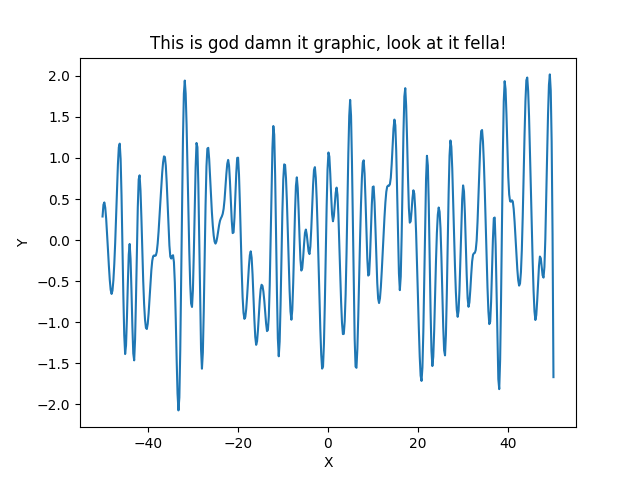
\includegraphics[scale=0.6]{function_graph.png} \end{figure}Alright fella, let's look wat we got:

\begin{equation}
{ln({{5}+{X}})}
\end{equation}
\begin{center} $\clubsuit$~$\clubsuit$~$\clubsuit$ \end{center}With the power of gods, let's write the following:
\begin{equation}
{ln({{5}+{X}})}
\end{equation}
\begin{center} $\clubsuit$~$\clubsuit$~$\clubsuit$ \end{center}I smacked a damn big cockroach yesterday fella, this was left on my shoe:
\begin{equation}
{{5}+{X}}
\end{equation}
\begin{center} $\clubsuit$~$\clubsuit$~$\clubsuit$ \end{center}Alright fella, let's make this shit called <Macloren>,there will be only 3 steps, cause i don't know how to count more.Basicly the main formula will look like that
 \[ f(x) = f(0) + \frac{f^{(1)}(0)}{1!}\cdot X + \frac{f^{(2)}(0)}{2!}\cdot X + \frac{f^{(3)}(0)}{3!}\cdot X + \text{...}\]
\[ f^{(0)}(0) = 1.60944\]\[ f^{(1)}(0) = 0.2\]\[ f^{(2)}(0) = -0.04\]\[ f^{(3)}(0) = 0.016\]
        The solution is pretty simple and you definetely can do it \textbf{yourself}
        \end{document}
    